\chapter{Quantum Entanglements, Part 1}

This lecture begins in a very controlled way. We are not asked, at first, to define entanglement in general. We are asked something more pointed: what difference can a sign make in a two-spin state? Susskind writes down two superpositions that look almost the same, insists that they are in fact quite different, and then unfolds the answer step by step. The route matters. We first rebuild the elementary spin algebra, then discover that one-spin observables do not distinguish the states at all, then find the right observable, and only after that widen the discussion to EPR correlation, Bell's inequality, projection operators, and no-cloning. These notes follow Leonard Susskind's lecture closely, with curation by LazyingArt LLC.

\section{Sign Choice in the Two-Spin State}

Let \(|u\rangle\) and \(|d\rangle\) denote the eigenstates of the third component of spin. For two spins we write
\[
|ud\rangle = |u\rangle_1\otimes |d\rangle_2,
\qquad
|du\rangle = |d\rangle_1\otimes |u\rangle_2,
\]
and from now on we suppress the tensor-product symbol in the lecture's style.

The opening puzzle is built from the two normalized states
\begin{equation}
|\psi_{\pm}\rangle
=
\frac{|ud\rangle \pm |du\rangle}{\sqrt{2}}.
\end{equation}
In both of them the third components are opposite. If one spin is up along the \(3\)-axis, the other is down; if one is down, the other is up. That much is common to both states. The normalization by \(\sqrt{2}\) is inserted immediately, because the discussion is about physical probabilities, not formal vectors only.

At this stage the two states sound nearly interchangeable. Both have the same up-down correlation in the third direction. But this is exactly Susskind's point: a sign that looks small in the formula can encode a large physical difference. We therefore do not begin by classifying the states abstractly; we begin by asking which calculations actually see that sign.

\section{Recalling the Pauli Actions and the Vanishing of One-Spin Averages}

Before answering the sign question, the lecture deliberately reinstalls the basic action table for the Pauli matrices. The pause is pedagogically important. The later manipulations will lean on these elementary actions over and over again.

\begin{figure}[h]
\centering

\includegraphics[width=0.42\textwidth]{lecture_05_figure_02.png}
\caption{The Pauli-action table being restarted on the board from the upper left corner.}
\end{figure}

We use
\begin{align}
\sigma_1|u\rangle &= |d\rangle, &
\sigma_1|d\rangle &= |u\rangle, \\
\sigma_2|u\rangle &= i|d\rangle, &
\sigma_2|d\rangle &= -i|u\rangle, \\
\sigma_3|u\rangle &= |u\rangle, &
\sigma_3|d\rangle &= -|d\rangle.
\end{align}
For the second electron we introduce another family \(\tau_1,\tau_2,\tau_3\), identical in algebra but acting on the second slot instead of the first.

Now comes the first important claim. In either of the states \( |\psi_+\rangle \) or \( |\psi_-\rangle \), every one-spin expectation value vanishes:
\begin{equation}
\langle \sigma_i\rangle = 0,
\qquad
\langle \tau_i\rangle = 0.
\end{equation}
So there is no direction in which either constituent spin is definitely polarized. This is already one of the characteristic signatures of the entangled state: whatever the total state may know, neither spin by itself carries a preferred direction.

\begin{figure}[h]
\centering

\includegraphics[width=0.60\textwidth]{lecture_05_figure_03.png}
\caption{The board layout for the entangled state and the claim that the one-spin expectation vanishes. The sign in the superposition is not fixed by the frame alone; the transcript shows that the explicit check here is done for the plus state.}
\end{figure}

\paragraph{A worked check.}
Susskind chooses the plus state for the explicit verification and checks \(\sigma_3\). We write
\begin{align}
\langle \psi_+|\sigma_3|\psi_+\rangle
&=
\frac{1}{2}
(\langle ud|+\langle du|)\sigma_3(|ud\rangle+|du\rangle).
\end{align}
Since \(\sigma_3\) acts on the first spin,
\[
\sigma_3|ud\rangle = |ud\rangle,
\qquad
\sigma_3|du\rangle = -|du\rangle.
\]
Therefore
\begin{align}
\langle \psi_+|\sigma_3|\psi_+\rangle
&=
\frac{1}{2}
(\langle ud|+\langle du|)(|ud\rangle-|du\rangle) \\
&=
\frac{1}{2}\bigl(\langle ud|ud\rangle-\langle du|du\rangle\bigr) \\
&=
\frac{1}{2}(1-1) \\
&= 0.
\end{align}
The cross terms vanish because \(\langle ud|du\rangle=\langle du|ud\rangle=0\). This is exactly the sort of explicit check the lecture insists on before moving on.

\subsection{Question \& Answer}

\paragraph{Question.} Does \(\langle \sigma_i\rangle = 0\) mean that the spin has eigenvalue \(0\)?

\paragraph{Answer.} No. For a single spin component the only possible outcomes are \(\pm 1\). There is no eigenstate of \(\sigma_i\) with eigenvalue \(0\). What vanishes is the expectation value. A measurement of one spin component in these states is a fair coin toss: up and down occur with equal probability.

That warning is not incidental. The lecture is already training us not to confuse an average statement with an outcome statement. If we flatten that distinction away, we lose the logic of what comes next.

\section{Total Spin, Singlet, and EPR Correlation}

Having shown that one-spin observables do not distinguish the two states, Susskind changes the question. We should not look at one little magnetic moment at a time; we should look at the sum of the two. The natural operators are
\[
\sigma_1+\tau_1,\qquad
\sigma_2+\tau_2,\qquad
\sigma_3+\tau_3.
\]

We begin with the third component. On the two basis states,
\begin{align}
(\sigma_3+\tau_3)|ud\rangle &= (1-1)|ud\rangle = 0, \\
(\sigma_3+\tau_3)|du\rangle &= (-1+1)|du\rangle = 0.
\end{align}
Therefore
\begin{equation}
(\sigma_3+\tau_3)(|ud\rangle \pm |du\rangle)=0.
\end{equation}
Both sign choices are eigenvectors of \(\sigma_3+\tau_3\) with eigenvalue \(0\). So the third component of the total spin still does not distinguish them.

The real difference appears when we move to the first component. Using the action table,
\begin{align}
(\sigma_1+\tau_1)|ud\rangle &= |dd\rangle + |uu\rangle, \\
(\sigma_1+\tau_1)|du\rangle &= |uu\rangle + |dd\rangle.
\end{align}
Hence
\begin{equation}
(\sigma_1+\tau_1)(|ud\rangle+|du\rangle)
=
2|uu\rangle+2|dd\rangle,
\end{equation}
while
\begin{equation}
(\sigma_1+\tau_1)(|ud\rangle-|du\rangle)=0.
\end{equation}
The plus state is not an eigenvector of \(\sigma_1+\tau_1\) with eigenvalue zero. The minus state is.

One should pause over that. The expectation value of the total first component may still vanish in the plus state, but the state is not annihilated by the operator. Consequently a measurement of the total first component need not return zero every time. Since each individual measurement gives \(\pm 1\), the sum can yield \(2\), \(0\), or \(-2\).

Now check the second component. Using
\[
\sigma_2|u\rangle = i|d\rangle,
\qquad
\sigma_2|d\rangle = -i|u\rangle,
\]
and the same for \(\tau_2\), we find
\begin{equation}
(\sigma_2+\tau_2)(|ud\rangle-|du\rangle)=0.
\end{equation}
Thus the minus-sign state is annihilated by all three components of the total spin. In compact notation,
\begin{equation}
(\boldsymbol{\sigma}+\boldsymbol{\tau})\cdot \hat n\,|\psi_-\rangle = 0
\qquad
\text{for every unit vector }\hat n.
\end{equation}

This is the special state of the lecture. The minus-sign state is the singlet. The plus-sign combination in this sector is the triplet. The singlet is rotationally invariant in the precise sense relevant here: no matter which component of the total spin we measure, the result is always zero.

The EPR correlation now falls straight out of the calculation. If Bob measures a component of one spin, he knows what Alice will get if she measures the same component of the other spin, because the sum of the two answers must vanish.

\subsection{Question \& Answer}

\paragraph{Question.} Is that statement only true on average?

\paragraph{Answer.} No. It is true every single time for the singlet, because the singlet is an eigenvector of the total spin component in every direction, with eigenvalue zero. The certainty comes from the eigenvector-eigenvalue relation, not merely from a statistical average.

\subsection{Question \& Answer}

\paragraph{Question.} Do these correlations violate causality, or allow signalling faster than light?

\paragraph{Answer.} No. Bob's measurement gives Bob information about what Alice would get if she measures the same component, but Alice's local statistics do not change. She still sees a fifty-fifty distribution. Only after Bob sends an ordinary classical message can she combine her result with his and recover the correlation. The correlation is immediate; the usable information is not.

This is why the lecture treats EPR correlation as profound but not as a direct violation of relativistic causality. It is deeper than the simple penny-and-dime example, because it works for every direction, but it does not by itself send messages.

\section{Bell's Inequality as a Classical Statement About Sets}

Only after the singlet and its correlation have been established does the lecture pivot to Bell. The pace changes intentionally. Susskind says he wants to go slowly, and the reason is clear: Bell's inequality must first be understood as an entirely classical theorem.

One may feel, as Susskind says Bell and Feynman sometimes did, that the theorem is either profoundly deep or almost trivial. But whatever attitude one takes toward its philosophy, the mathematical statement itself is classical. Classical logic here means set theory.

Suppose we have a set of objects, each of which may or may not possess three properties \(A\), \(B\), and \(C\). Then Bell's inequality is the counting statement
\begin{equation}
N(A,\neg B)+N(B,\neg C)\ge N(A,\neg C).
\end{equation}
Here \(N(A,\neg B)\) means the number of objects that have property \(A\) and do not have property \(B\), and similarly for the other terms.

Susskind wants a picture, not a ceremonial proof. We should see the theorem in the geometry of subsets.

\begin{figure}[h]
\centering
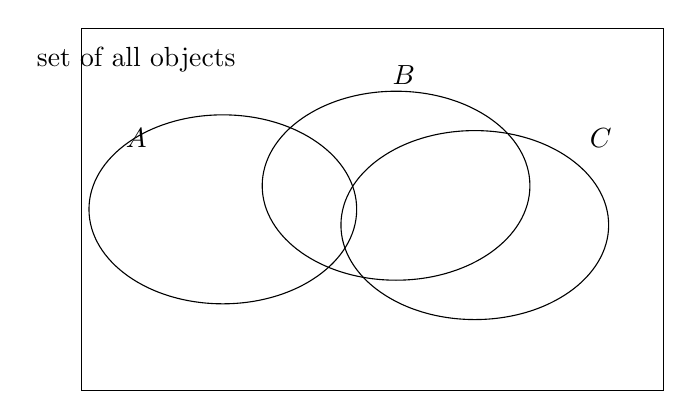
\begin{tikzpicture}[scale=1.0]
\draw (-3.7,-2.3) rectangle (3.7,2.3);
\node at (-3.0,1.9) {set of all objects};
\draw (-1.9,0.0) ellipse (1.7 and 1.2);
\draw (0.3,0.3) ellipse (1.7 and 1.2);
\draw (1.3,-0.2) ellipse (1.7 and 1.2);
\node at (-3.0,0.9) {$A$};
\node at (0.4,1.7) {$B$};
\node at (2.9,0.9) {$C$};
\end{tikzpicture}
\caption{A classical picture of the properties \(A\), \(B\), and \(C\) as subsets of a set.}
\end{figure}

One clean way to express the content is
\[
A\cap \neg C
\subset
(A\cap \neg B)\cup(B\cap \neg C).
\]
Indeed, if an object lies in \(A\cap \neg C\), then either it has \(B\) or it does not. If it does not have \(B\), it lies in \(A\cap \neg B\). If it does have \(B\), then together with \(\neg C\) it lies in \(B\cap \neg C\). Taking cardinalities gives the inequality.

This is classical from start to finish. No noncommuting observables, no amplitudes, no Hilbert space. The lecture is careful about this because the later violation should be seen as a failure of classical set-theoretic reasoning in the quantum context, not as a cheat in the derivation.

\section{From Spin Propositions to Projection Operators}

We now specialize the abstract properties \(A\), \(B\), and \(C\) to propositions about the singlet pair. Following the lecture, we define
\begin{align}
A &: \text{spin 1 is up at }0^\circ, \text{ that is, along the }3\text{-axis}, \\
B &: \text{spin 1 is up at }45^\circ \text{ in the }zx\text{-plane}, \\
C &: \text{spin 1 is up at }90^\circ \text{ in the same plane}.
\end{align}
The transcript hesitates briefly about the plane, but the subsequent algebra fixes it: the intended plane is the \(zx\)-plane.

\begin{figure}[h]
\centering
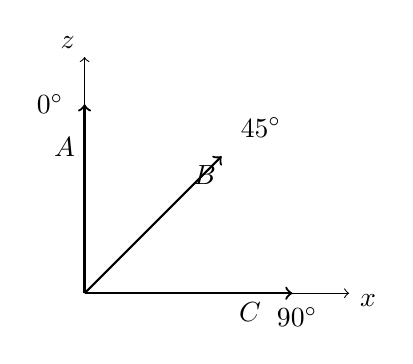
\begin{tikzpicture}[scale=1.2]
\draw[->] (0,0)--(0,2.5);
\draw[->] (0,0)--(2.8,0);
\node at (-0.18,2.65) {$z$};
\node at (3.0,-0.08) {$x$};
\draw[thick,->] (0,0)--(0,2.0);
\draw[thick,->] (0,0)--(1.45,1.45);
\draw[thick,->] (0,0)--(2.2,0);
\node[left] at (0,1.55) {$A$};
\node[above right] at (1.05,1.05) {$B$};
\node[below] at (1.75,0) {$C$};
\node[left] at (-0.12,2.0) {$0^\circ$};
\node[above right] at (1.55,1.55) {$45^\circ$};
\node[below] at (2.25,-0.05) {$90^\circ$};
\end{tikzpicture}
\caption{The three directions used in the Bell discussion.}
\end{figure}

Because the state is the singlet, the negation of a proposition about spin 1 becomes a positive proposition about spin 2. Thus \(\neg B\) may be read as: spin 2 is up at \(45^\circ\). Likewise \(\neg C\) becomes: spin 2 is up at \(90^\circ\).

At this point the lecture asks the practical question that forces the next construction: how do we actually compute the relevant probabilities? This is the moment where projection operators enter.

\begin{figure}[h]
\centering

\includegraphics[width=0.58\textwidth]{lecture_05_figure_04.png}
\caption{The lecture's geometric and algebraic introduction to projection operators.}
\end{figure}

The generic board equation is only partly legible, so we write it in cautious standard form:
\begin{equation}
P|\alpha\rangle = |\alpha_p\rangle.
\end{equation}
The meaning is plain from the diagram: \(P\) projects the vector \(|\alpha\rangle\) onto a chosen subspace and removes the component orthogonal to that subspace.

\begin{figure}[h]
\centering
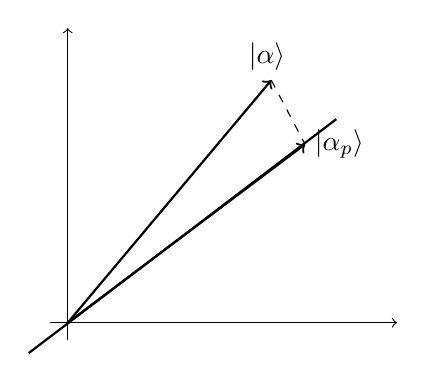
\begin{tikzpicture}[scale=1.1]
\draw[->] (-0.2,0)--(3.8,0);
\draw[->] (0,-0.2)--(0,3.4);
\draw[thick] (-0.45,-0.35)--(3.1,2.35);
\draw[->,thick] (0,0)--(2.35,2.8);
\node[above] at (2.3,2.8) {$|\alpha\rangle$};
\draw[dashed] (2.35,2.8)--(2.74,2.06);
\draw[->,thick] (0,0)--(2.74,2.06);
\node[right] at (2.74,2.06) {$|\alpha_p\rangle$};
\end{tikzpicture}
\caption{A clean redraw of the projection geometry used in the lecture.}
\end{figure}

Susskind then specializes to the one-spin space. If we project onto the subspace where the third component is \(+1\), then the down component is simply discarded:
\begin{equation}
P_{\sigma_3=+1}
\begin{pmatrix}
\alpha \\ \beta
\end{pmatrix}
=
\begin{pmatrix}
\alpha \\ 0
\end{pmatrix},
\qquad
P_{\sigma_3=-1}
\begin{pmatrix}
\alpha \\ \beta
\end{pmatrix}
=
\begin{pmatrix}
0 \\ \beta
\end{pmatrix}.
\end{equation}

\begin{figure}[h]
\centering

\includegraphics[width=0.58\textwidth]{lecture_05_figure_05.png}
\caption{Projection onto the \(\sigma_3=\pm 1\) subspaces and the move toward matrix form.}
\end{figure}

The operator itself is
\begin{equation}
P_{\sigma_3=+1}
=
\begin{pmatrix}
1 & 0 \\
0 & 0
\end{pmatrix}
=
\frac{1+\sigma_3}{2}.
\end{equation}
And more generally, for any unit vector \(\hat n\),
\begin{equation}
P_{\sigma\cdot \hat n = +1}
=
\frac{1+\sigma\cdot \hat n}{2}.
\end{equation}
The probability postulate can now be stated in the form used by the lecture:
\begin{equation}
\mathrm{Prob}(\alpha\ \text{true in the state }|\psi\rangle)
=
\langle \psi|P_\alpha|\psi\rangle.
\end{equation}

For the Bell quantity \(A\wedge \neg B\), the first statement is ``spin 1 is up at \(0^\circ\),'' and the second, after the singlet reinterpretation, is ``spin 2 is up at \(45^\circ\).'' Therefore
\begin{equation}
P_{A\wedge \neg B}
=
\frac{1+\sigma_3}{2}\,
\frac{1+\tau\cdot \hat n_{45}}{2},
\qquad
\hat n_{45}=\frac{\hat x+\hat z}{\sqrt{2}},
\qquad
\tau\cdot \hat n_{45}=\frac{\tau_1+\tau_3}{\sqrt{2}}.
\end{equation}

\subsection{Question \& Answer}

\paragraph{Question.} Why does the product of projectors represent the logical word ``and''?

\paragraph{Answer.} Only when the propositions are compatible, meaning that their projectors commute. For one electron, the statements ``spin up along the \(3\)-axis'' and ``spin up along the \(1\)-axis'' are not jointly meaningful in this way, because the corresponding projectors do not commute. Here, however, one projector acts on spin 1 and the other on spin 2. The \(\sigma\)'s commute with the \(\tau\)'s, so the product does define the conjunction.

This clarification comes late in the lecture, but it is structurally important. Without it the Bell computation looks more classical than it really is.

\section{Quantum Violation of Bell's Inequality}

Now the lecture turns the machinery on. Let
\begin{equation}
|\psi_s\rangle
=
\frac{|ud\rangle-|du\rangle}{\sqrt{2}}
\end{equation}
be the singlet state.

Susskind first notes the qualitative result: the quantum value of the left-hand side of Bell's inequality will come out smaller than the right-hand side. Then he says the only thing to do is to hold one's breath and compute.

\paragraph{The probability \(P(A,\neg B)\).}
We evaluate
\[
P(A,\neg B)=\langle \psi_s|P_{A\wedge \neg B}|\psi_s\rangle.
\]
Act first with \((1+\sigma_3)/2\). This projects onto the component where the first spin is up, so it kills the \(|du\rangle\) term and leaves
\[
\frac{1}{\sqrt{2}}|ud\rangle.
\]
Now act with the second projector:
\begin{align}
\frac{1+\tau\cdot \hat n_{45}}{2}|ud\rangle
&=
\frac{1}{2}
\left(
|ud\rangle
+
\frac{\tau_1+\tau_3}{\sqrt{2}}|ud\rangle
\right) \\
&=
\frac{1}{2}
\left(
|ud\rangle
+
\frac{|uu\rangle-|ud\rangle}{\sqrt{2}}
\right).
\end{align}
So
\begin{equation}
\frac{1+\tau\cdot \hat n_{45}}{2}|ud\rangle
=
\frac{1}{2}
\left(
\left(1-\frac{1}{\sqrt{2}}\right)|ud\rangle
+
\frac{1}{\sqrt{2}}|uu\rangle
\right).
\end{equation}
When we now take the inner product with the singlet bra, the \(|uu\rangle\) term does not contribute, because it is orthogonal to both \(\langle ud|\) and \(\langle du|\). The surviving piece is therefore
\begin{equation}
P(A,\neg B)
=
\frac{1}{4}\left(1-\frac{1}{\sqrt{2}}\right).
\end{equation}

The lecture does not recompute \(P(B,\neg C)\) from scratch. Instead it uses rotational invariance of the singlet. The two situations differ only by a \(45^\circ\) rotation, so
\begin{equation}
P(B,\neg C)
=
\frac{1}{4}\left(1-\frac{1}{\sqrt{2}}\right).
\end{equation}

\paragraph{The probability \(P(A,\neg C)\).}
Now \(\neg C\) becomes the statement that spin 2 is up at \(90^\circ\), that is, along the \(1\)-axis. Thus the projector is
\[
\frac{1+\sigma_3}{2}\,\frac{1+\tau_1}{2}.
\]
As before, the first factor kills \(|du\rangle\) and leaves \(|ud\rangle/\sqrt{2}\). Then
\begin{equation}
\frac{1+\tau_1}{2}|ud\rangle
=
\frac{1}{2}(|ud\rangle+|uu\rangle).
\end{equation}
The \(|uu\rangle\) term again has zero overlap with the singlet bra, so
\begin{equation}
P(A,\neg C)=\frac{1}{4}.
\end{equation}

Putting the three numbers together,
\begin{equation}
P(A,\neg B)+P(B,\neg C)
=
\frac{1}{2}\left(1-\frac{1}{\sqrt{2}}\right)
<
\frac{1}{4}
=
P(A,\neg C).
\end{equation}
Numerically,
\[
\frac{1}{2}\left(1-\frac{1}{\sqrt{2}}\right)\approx 0.146,
\qquad
\frac{1}{4}=0.25.
\]
The decimal estimates in the lecture are informal, but the exact algebraic comparison is clean.

What is the meaning of the violation? The lecture's answer is blunt: there is no underlying classical description in which quantum propositions are governed by ordinary set theory. Quantum mechanics is not the statistical mechanics of some unseen classical system whose properties obey classical logic all the way down.

This is where Aspect's experiment enters. Susskind is careful about what it did and did not establish. It did not decide whether quantum mechanics works in general; that was already known. What it sharpened was the locality issue. By arranging the measurements so that no light-speed signal could pass from one wing of the experiment to the other in time, it blocked the obvious classical escape route in which hidden information travels from left to right. The achievement was as much one of timing and experimental control as of principle.

\section{Linearity and the No-Cloning Theorem}

The final turn of the lecture is abrupt but natural. After Bell and the discussion of compatible projectors, Susskind decides to postpone the measurement problem and instead prove a short theorem. The new input is the linearity of quantum evolution:
\begin{equation}
|a\rangle\to |a'\rangle,
\qquad
|b\rangle\to |b'\rangle
\quad \Longrightarrow \quad
\alpha|a\rangle+\beta|b\rangle
\to
\alpha|a'\rangle+\beta|b'\rangle.
\end{equation}
Superpositions evolve into superpositions with the same coefficients.

Now imagine a machine that clones quantum states. At minimum it would have to work on the \(u/d\) basis:
\begin{equation}
|u\rangle \to |uu\rangle,
\qquad
|d\rangle \to |dd\rangle.
\end{equation}
Next define the state pointing to the right,
\begin{equation}
|r\rangle=\frac{|u\rangle+|d\rangle}{\sqrt{2}}.
\end{equation}
If the same machine were universal, then by linearity its output on \(|r\rangle\) would be forced to be
\begin{equation}
|r\rangle \to \frac{|uu\rangle+|dd\rangle}{\sqrt{2}}.
\end{equation}
But exact cloning would require two independent copies of \(|r\rangle\):
\begin{align}
|rr\rangle
&=
|r\rangle\otimes |r\rangle \\
&=
\frac{1}{2}
\bigl(
|uu\rangle+|ud\rangle+|du\rangle+|dd\rangle
\bigr).
\end{align}
These are different states. The linear output has only the two parallel terms \(|uu\rangle\) and \(|dd\rangle\). The genuinely cloned state necessarily contains the mixed terms \(|ud\rangle\) and \(|du\rangle\) as well.

\begin{theorem}[No-cloning]
A single machine cannot clone an arbitrary unknown quantum state.
\end{theorem}

\begin{proof}
Assume one machine clones \(|u\rangle\) and \(|d\rangle\), so that
\[
|u\rangle \to |uu\rangle,
\qquad
|d\rangle \to |dd\rangle.
\]
By linearity, the same machine must send
\[
\frac{|u\rangle+|d\rangle}{\sqrt{2}}
\to
\frac{|uu\rangle+|dd\rangle}{\sqrt{2}}.
\]
But exact cloning of the input state would require
\[
\left(\frac{|u\rangle+|d\rangle}{\sqrt{2}}\right)
\otimes
\left(\frac{|u\rangle+|d\rangle}{\sqrt{2}}\right)
=
\frac{1}{2}
\bigl(
|uu\rangle+|ud\rangle+|du\rangle+|dd\rangle
\bigr).
\]
Since these outputs are different, the supposed universal cloning machine cannot exist.
\end{proof}

The lecture does not state the moral sloppily. If the state is known in advance, one can design a device adapted to that state or to a chosen basis. What cannot be done is to build a single machine that clones everything. Cloning is effectively quadratic in the state, while quantum evolution is linear. That mismatch is the whole theorem in a nutshell.

\section{Summary}

The lecture opens with a sign and spends its first half earning the right to say why the sign matters. For the states
\[
\frac{|ud\rangle\pm|du\rangle}{\sqrt{2}},
\]
every one-spin expectation value vanishes, so no difference appears at the level of either spin separately. The distinction emerges only when we look at the total spin. The minus-sign state is the singlet, annihilated by every component of \(\sigma+\tau\), and therefore perfectly anti-correlated in every direction.

From there the lecture broadens without losing the thread. Bell's inequality is introduced as a classical counting theorem, then translated into the singlet experiment, and then violated by an explicit projector calculation. The meaning of that violation is not that quantum mechanics is inconsistent, but that its propositions do not live inside ordinary set theory. The closing theorem makes the same Hilbert-space structure felt in another way: because quantum evolution is linear, no universal machine can clone an arbitrary unknown state. The lecture has unfolded one theme through several faces. A sign, a correlation, a violated inequality, and a no-go theorem are all part of the same quantum geometry.